\begin{figure}
  \centering
  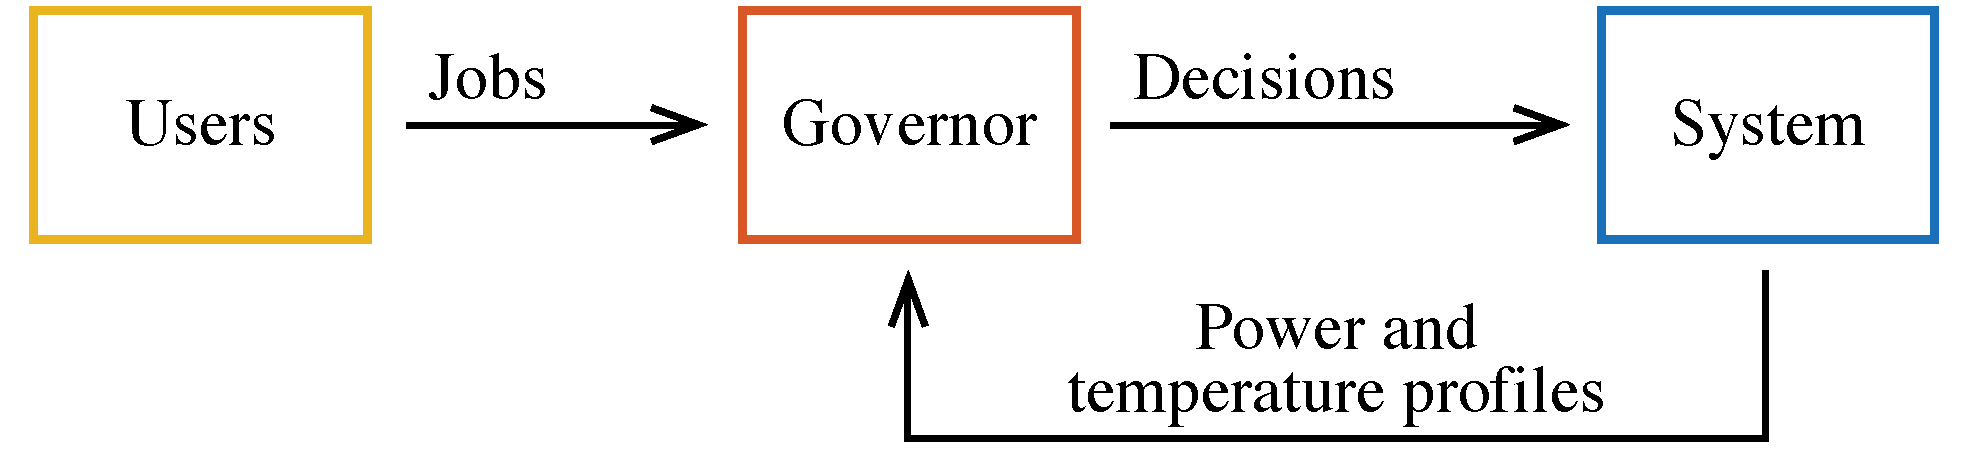
\includegraphics[width=1.0\columnwidth]{include/assets/figures/usage.pdf}
  \caption{A usage example with a feedback loop.}
  \flab{usage}
\end{figure}

\begin{table}
  \caption{Target architecture}
  \begin{tabular*}{\linewidth}{=L{70pt}l}
    \toprule
    Component    & Description \\
    \midrule
    Core         & 2660 MHz, 1.2 V \\
    L1-I/D cache & 32 KB, 4-way, LRU, private \\
    L2 cache     & 256 KB, 4-way, LRU, private \\
    L3 cache     & 8192 KB, 16-way, LRU, one per four cores \\
    \bottomrule
  \end{tabular*}
  \tlab{target}
\end{table}
% vim: nowrap tw=0

Before concluding the paper, we would like to illustrate how one can approach
acquiring reference arrival and workload data and to discuss two common schemes
of integrating the methodology into the workflow of a research project.

In order to get real-life arrival patterns, we used a dataset published by
Google \cite{google}. The dataset contains usage data of a computer cluster over
a month period, namely, over May 2011. We processed the table that was tracking
the life cycles of the jobs submitted to the cluster and extracted the time
stamps of the first event related to each job. As a result, we obtained almost
670,000 arrivals, which we used for model fitting as it was described
\sref{traffic}. The described processing scheme is rather straightforward and
could be a good place to start. However, one can perform a more sophisticated
filtration in order to distill more specific and accurate information.

The workload patterns are obtained by simulating applications from two widely
used benchmark suites, namely, from \sc{PARSEC} \cite{bienia2011} and \sc{SPEC
CPU2006} \cite{cpu2006}.

A usage example with a feedback loop is given in \fref{usage}. Our methodology
revolves about the box in the middle and provides the boxes to the sides.
